% ---------------------------------------------------------------------------
\section{Data Cleaning}
\label{sec:cleaning}
% ---------------------------------------------------------------------------

The training file contains 7,829 missing cells across nineteen attributes, but the
count alone is misleading. Figure~\ref{fig:missing} shows a characteristic pattern:
the largest gaps belong to features that most houses simply do not have. A pool
quality is missing for 1,453 of 1,460 properties, a miscellaneous feature for 1,406,
an alley for 1,369 and a fence for 1,179. Imputing a mode into these columns would
invent amenities that do not exist; the correct treatment records absence as a level.

\begin{figure}[htbp]
\centering
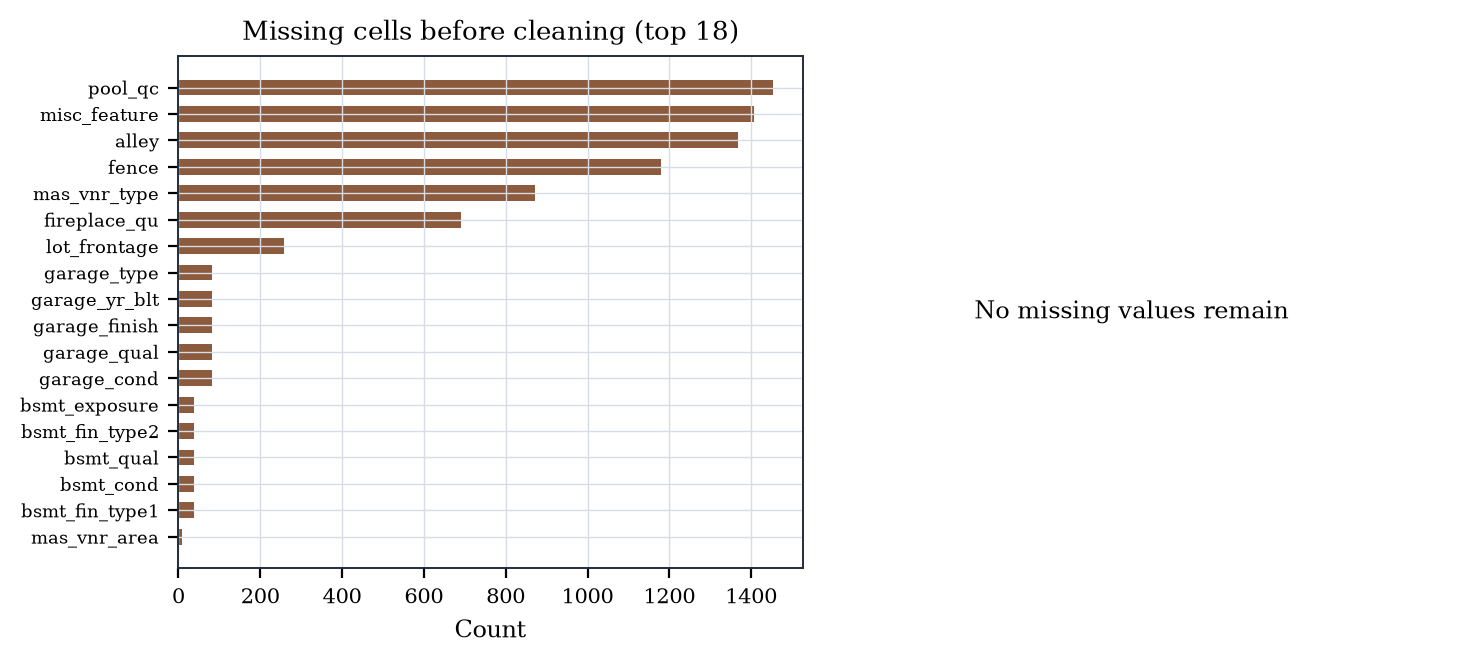
\includegraphics[width=0.86\linewidth]{fig07_missing_values.png}
\caption{Missing cells by attribute before cleaning (eighteen most affected
attributes) and the confirmation that no missing values remain after the rules are
applied.}
\label{fig:missing}
\end{figure}

Three semantics are present, and distinguishing them is the conceptual work of this
module. \emph{Structural absence} means the property does not have the feature, and
the missing value is information: a house without a basement has no basement quality.
\emph{Absent quantity} means the feature exists conceptually but has zero extent: a
house with no garage has zero garage area. \emph{Genuine missingness} means the value
exists but was not recorded, which is the case for lot frontage on 259 properties and
the electrical system on one. Table~\ref{tab:cleaning} records the treatment for each
group.

\begin{table}[htbp]
\centering
\caption{Missing-data treatment by semantic group. Counts refer to the training file.
The total of 7,829 cells is reduced to zero and no row is dropped for missingness.}
\label{tab:cleaning}
\small
\begin{tabularx}{\linewidth}{@{}L{0.22\linewidth}L{0.27\linewidth}rL{0.24\linewidth}@{}}
\toprule
\textbf{Group} & \textbf{Attributes} & \textbf{Cells} & \textbf{Treatment} \\
\midrule
Structural absence & 15 attributes (pool, alley, fence, basement and garage quality, fireplace quality, veneer type) & 7,480 & Literal level ``None'' \\
Absent quantity & Masonry veneer area & 8 & Zero \\
Unstructured categorical & Electrical system & 1 & Training mode \\
Lot frontage & Continuous & 259 & Neighbourhood median, global fallback \\
Garage year & Construction year & 81 & House construction year \\
\midrule
Total & 19 attributes & 7,829 & No missing cells remain \\
\bottomrule
\end{tabularx}
\end{table}

Lot frontage is imputed by neighbourhood rather than globally for a reason. Frontage
is strongly related to neighbourhood type, and the neighbourhood medians range from
21 feet in MeadowV and BrDale to 91 feet in NoRidge. A global median of 69 feet would
assign the same frontage to a dense inner-suburb lot and to a large estate lot, and
would therefore attenuate the relationship between frontage and price.

Outliers are handled by five explicit rules: implausible area--price combinations
(more than 4,000 square feet sold below 300,000 \USD), extreme lot size (above
100,000 square feet), implausible price per square foot (outside 25--500 \USD),
invalid garage year and invalid remodelling year. Only the first removes records: two
transactions, 0.14 per cent of the sample, which are inconsistent with the local
price-per-square-foot distribution and exert disproportionate leverage on a
least-squares fit. The removal applies to training data only; the unlabelled file is
scored in full. The extreme-lot rule flags four observations but removes none,
because a large lot is a genuine market feature rather than a data-entry error, and
the remaining three rules found no violations.

The decision to retain the 61 interquartile-range price outliers (4.2 per cent of the
sample) is equally deliberate. These are expensive houses, not erroneous records, and
deleting them would bias the model against precisely the luxury segment that the
subgroup analysis later identifies as weakest. The log transformation already limits
their influence, and conformal calibration absorbs their effect on interval width.
Removing them would improve the reported average error while making the product worse
for the customers who need it most.

The duplicate check found no exact duplicate records and no duplicated transaction
identifiers, leaving 1,458 rows from the original 1,460. Categorical labels were
canonicalised before validation: whitespace stripped and collapsed, case folded, and
documented spelling variants mapped to a canonical level. No residual inconsistency
survived this pass in the training file, which is reported as zero label variants
fixed. Unknown levels are preserved rather than coerced to the mode, so a genuinely
new category in the unlabelled file does not silently become a frequent one, and the
same mapping is applied at inference time. Every decision in this section is recorded
in \texttt{artifacts/metrics/cleaning\_report.json}, including per-attribute counts,
the neighbourhood medians used for imputation and the rule text for each outlier
check, so the before-and-after comparison can be verified rather than trusted.
